\section{Logical Design}

\subsection{Transformation of the Entity-Relationship Schema}


\subsubsection{Redundancy Analysis}
\begin{itemize}
	\item The proposed ER Schema does not have any external identifier.
	\item The proposed ER Schema does not have any relationship cycles.
	\item The proposed ER Schema does not have any derivated attributes.
\end{itemize}

\subsubsection{Choice of Principal Identifiers}
By checking the graph of the (main) external identifiers, it appears that the scheme does 
not have external identification cycles, furthermore the main identifiers respect the selection criteria.
\subsection{Analysis of Database Load}
The finance team wants to know the repairments number for each used car in order to deduce the convenience of keeping or not the car for rent option.\\ 
We compute the load analysis to decide whether to introduce or not the \#repairs: a derived attribute for the UsedCar entity to quickly check how many repairs a car underwent.\\ 
We studied an example considering 10000 instances of repairs and 50 of used cars.

\newpage

\begin{longtable}{|p{.25\columnwidth}|p{.45\columnwidth}|p{.1\columnwidth}|p{.1\columnwidth}|}
	\hline
	\textbf{Operation} & \textbf{Description} & \textbf{Frequency} & \textbf{Type} \\
	\hline 
	\centering{O$_1$} \\ Insert new repair & Store data about a new repair coming from a UsedCar & 100/month & Online \\
	\hline
	\centering{O$_2$} \\ Repair list & Print the list of the repair from a UsedCar & 1/month & Online \\
	\hline
\end{longtable}

\textbf{If we have no redundancy:}
\begin{itemize}
\item in the O$_1$ operation: 
\begin{longtable}{|p{.2\columnwidth}|p{.2\columnwidth}|p{.1\columnwidth}|p{.1\columnwidth}|p{.20\columnwidth}|}
	\hline
	\textbf{Concept} & \textbf{Construct} & \textbf{Access} & \textbf{Type} & \textbf{Average Access} \\
	\hline 
	Repair & Entity & 1 & W & 1x100x2 = 200 \\
	\hline
	UsedRepairs & Relationship & 1 & W & 1x100x2 = 200 \\
	\hline 
	\multicolumn{4}{|c|}{Total Access} & \multicolumn{1}{c|}{400} \\
	\hline
\end{longtable}
\item in the O$_2$ operation: 
\begin{longtable}{|p{.2\columnwidth}|p{.2\columnwidth}|p{.1\columnwidth}|p{.1\columnwidth}|p{.20\columnwidth}|}
	\hline
	\textbf{Concept} & \textbf{Construct} & \textbf{Access} & \textbf{Type} & \textbf{Average Access} \\
	\hline 
	UsedCar & Entity & 1 & R & 1x1x1 = 1 \\
	\hline
	UsedRepairs & Relationship & 200 & R & 200x1x1 = 200 \\
	\hline
	\multicolumn{4}{|c|}{Total Access} & \multicolumn{1}{c|}{201} \\
	\hline
\end{longtable}
\vspace{-0.3cm}
So, in the end we get an amount of access equal to 601. 
\end{itemize}

\textbf{If we have \#repairs attribute:} 
\begin{itemize}
\item in the O$_1$ operation: 
\begin{longtable}{|p{.2\columnwidth}|p{.2\columnwidth}|p{.1\columnwidth}|p{.1\columnwidth}|p{.20\columnwidth}|}
	\hline
	\textbf{Concept} & \textbf{Construct} & \textbf{Access} & \textbf{Type} & \textbf{Average Access} \\
	\hline 
	Repair & Entity & 1 & W & 1x100x2 = 200 \\
	\hline
	UsedRepairs & Relationship & 1 & W & 1x100x2 = 200 \\
	\hline 
	UsedCar & Entity & 1 & R & 1x100x1 = 100 \\ 
	\hline 
	UsedCar & Entity & 1 & W & 1x100x2 = 200 \\ 
	\hline
	\multicolumn{4}{|c|}{Total Access} & \multicolumn{1}{c|}{700} \\
	\hline
\end{longtable}
\item in the O$_2$ operation: 
\begin{longtable}{|p{.2\columnwidth}|p{.2\columnwidth}|p{.1\columnwidth}|p{.1\columnwidth}|p{.20\columnwidth}|}
	\hline
	\textbf{Concept} & \textbf{Construct} & \textbf{Access} & \textbf{Type} & \textbf{Average Access} \\
	\hline 
	UsedCar & Entity & 1 & R & 1x1x1 = 1 \\ 
	\hline 
	\multicolumn{4}{|c|}{Total Access} & \multicolumn{1}{c|}{1} \\
	\hline
\end{longtable}
\vspace{-0.3cm}
So, in the and we get an amount of access equal to 701.
\end{itemize}

\noindent The \#repairs attribute did not significantly improves the operations performances. For this reason, we decided not keep the redundant attribute in our schema. 



\subsection{Relational Schema}
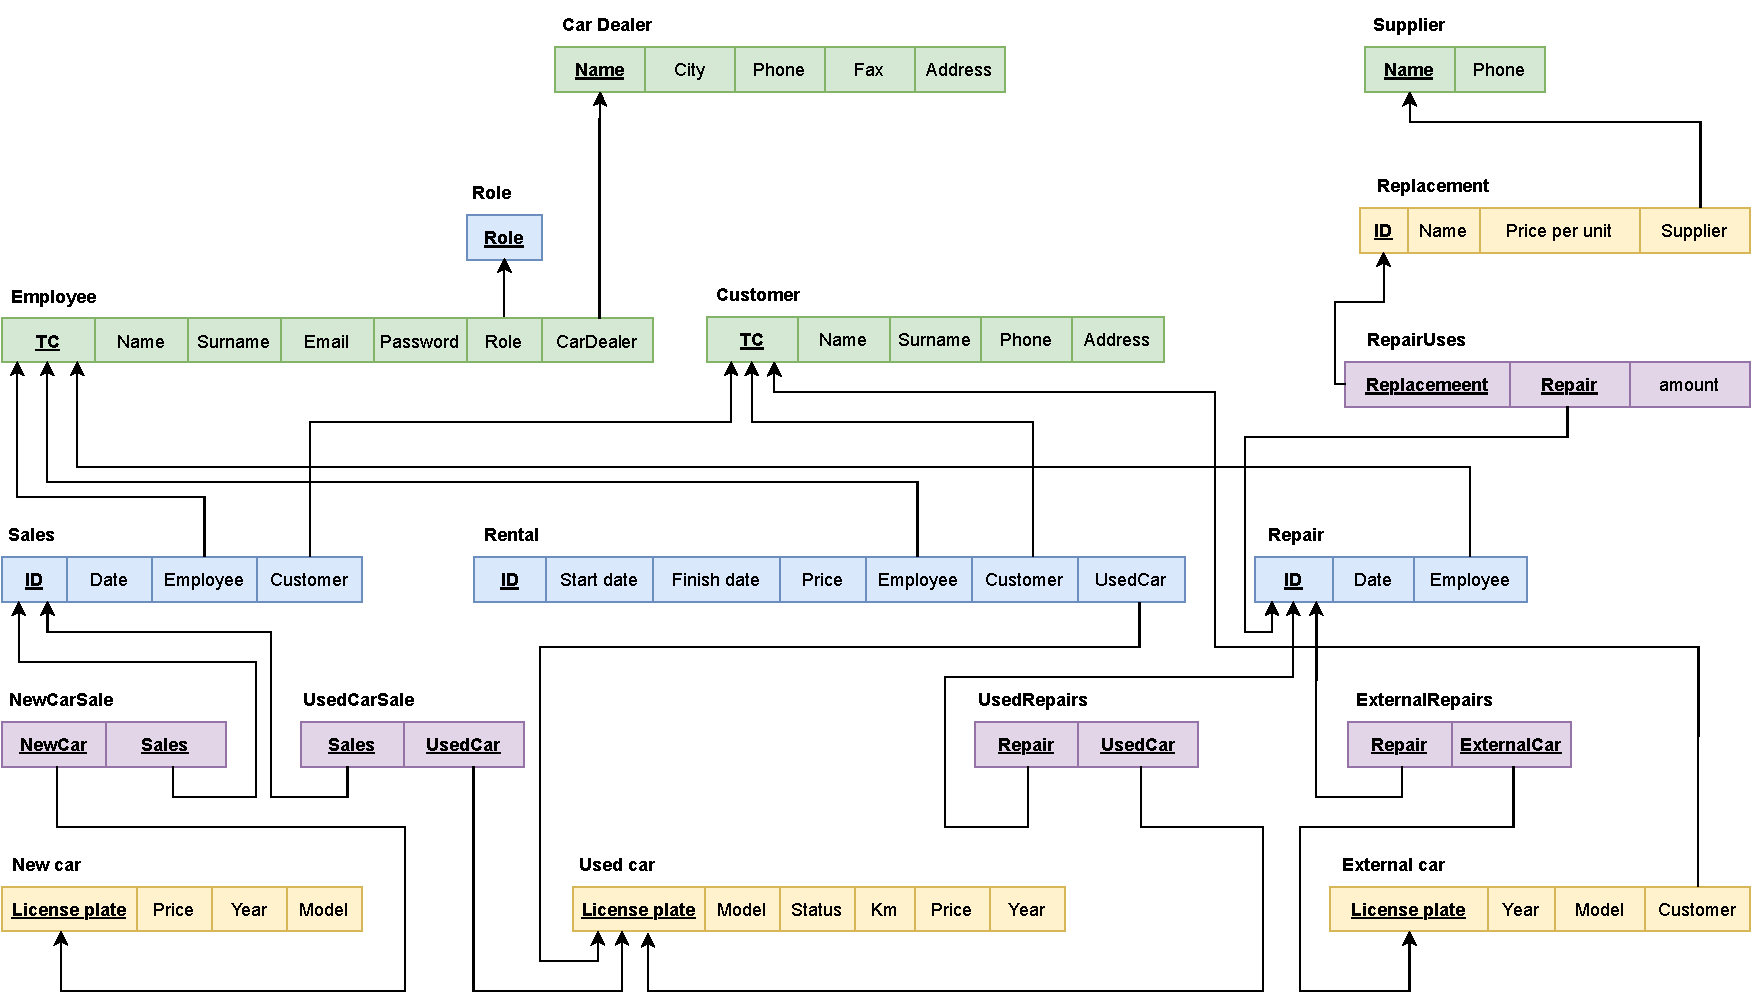
\includegraphics[scale=0.55]{relational_schema}

NewCarSale, UsedCarSale, UsedRepairs and ExternalRepairs are relationships with optional partecipation, thus two options are available when converting them to relations:
\begin{enumerate}
	\item Create a new relation which references (with a foreign key constraint) the two participants in the relationship.
	\item Incorporate the references in the relations Sales and Repair.
\end{enumerate}
The second option is simpler (because we don't need to introduce 4 extra relations) but it is also less efficient, since each instance of Repair and Sales is going to contain a null value. While this choice could be acceptable for an infrequently used relation, it is not tolerable in our case. For this reason it was decided to adopt the first solution.
All the other relationships can be converted straightforwardly.

\subsection{Data Dictionary}

\begin{longtable}{|p{.15\columnwidth}|p{.15\columnwidth} |p{.30\columnwidth}|p{.10\columnwidth}|p{.20\columnwidth} |} 
\hline
\textbf{Relation} & \textbf{Attribute} & \textbf{Description} & \textbf{Domain} & \textbf{Constraints} \\\hline

\multirow{4}{*}{Sales}
    & ID & Identifier of the sale & Serial & Primary key \\\cline{2-5}
    & Date & Date at which the sale was performed & Datetime & Not Null\\\cline{2-5}
    & Employee & Identifier of the employee & Text & Foreign key to Employee\\\cline{2-5}
    & Customer & Identifier of the customer & Text & Foreign key to Customer\\\hline

\multirow{2}{*}{New Car Sale} 
    & NewCar & Identifier of the New Car & Text & Foreign key to New Car, Primary key with ID \\\cline{2-5}
    & Sales & Identifier of the sale & Serial & Foreign key to Sales, Primary key with NewCar\\\hline

\multirow{4}{*}{NewCar}
    & License Plate & Identifier of the New Car & Text & Primary key \\\cline{2-5} 
    & Price & Price of the car & Float & Not Null \\\cline{2-5}
    & Year & Year of registration of the car & Smallint & Not Null \\\cline{2-5}
    & Model & Model of the car & Text & Not Null \\\hline

\multirow{2}{*}{Used Car Sale} 
    & Sales & Identifier of the sale & Serial & Foreign key to Sales\\\cline{2-5}
    & UsedCar & Identifier of the Used Car & Text & Foreign key to Used Car \\ \hline

\multirow{7}{*}{Used Car}
    & License Plate & Identifier of the Used Car & Text & Primary key \\\cline{2-5}
    & Model & Model of the car & Text & Not Null \\\cline{2-5} 
    & Status & Status of the car & Text & Not Null\\\cline{2-5}
    & Km & Mileage of the car & Int & Not Null \\\cline{2-5}
    & Price & Price referred to the sale of the used vehicle & Float & Not Null \\\cline{2-5} 
    & Year & Year of the car & Smallint & Not Null \\ \hline

\multirow{5}{*}{Customer}
    & TC & Identifier of the customer & Text & Primary key \\\cline{2-5}
    & Name & Name of the customer & Text & Not Null \\\cline{2-5}
    & Surname & Surname of the customer & Text & Not Null \\\cline{2-5}
    & Phone & Phone number of the customer & Text & Not Null \\\cline{2-5}
    & Address &  Residential address of the client & Text & Not Null \\\hline

\multirow{5}{*}{Car Dealer} 
    & Name & Branch name of the car dealer & Text & Primary key \\\cline{2-5}
    & City & City where the branch is located & Text & Not Null \\\cline{2-5}  
    & Phone & Phone number associated to the branch & Text & Not Null \\\cline{2-5}  
    & Fax & Fax number & Text & \\\cline{2-5}
    & Address & Address of the branch & Text & Not Null \\\hline

\multirow{7}{*}{Employee} 
    & TC & Identifier of the employee & Text & Primary key \\\cline{2-5} 
    & Name & Name of the employee & Text & Not Null \\\cline{2-5}
    & Surname & Surname of the employee & Text & Not Null \\\cline{2-5}
    & Email & Email of the employee used to access the management system & Text & Not Null \\\cline{2-5}
    & Password & Password needed by the employee to access the management system & Text & Not Null \\\cline{2-5}
    & Role & Identifier of a Role & Text & Foreign key to Role\\\cline{2-5}
    & Car Dealer & Branch name of the car dealer & Text & Foreign Key to Car Dealer \\\hline

\multirow{2}{*}{Role} 
    & Role Name & Identifier of a Role & Text & Primary key \\\cline{2-5}
    \\\hline

\multirow{6}{*}{Rental} 
    & Rental ID  & Identifier of a Rent & Serial & Primary key \\\cline{2-5}
    & Start Date & Date from which the Rental starts & Text & Not Null\\\cline{2-5}
    & Finish Date & Date at which the Rental finished & Text & \\\cline{2-5}
    & Employee & Identifier of the employee & Text & Foreign key to Employee\\\cline{2-5}
    & Customer & Identifier of the customer & Text & Foreign key to Customer\\\cline{2-5}
    & Price & Rental price related & Float & Not Null\\\cline{2-5}
    & Used Car & Identifier of the Used Car & Text & Foreign key to UsedCar\\\hline

\multirow{4}{*}{Used Repairs} 
    & Repair & Identifier to Repair & Serial & Foreign key to Repair, Primary key with Used Car\\\cline{2-5}
    & UsedCar & Identifier of the Used Car & Text & Foreign key to External Car, Primary key with Repair\\\hline

\multirow{3}{*}{Repair}  
    & ID & Identifier of Repair & Serial & Primary key \\\cline{2-5}
    & Date & Date at which the Repair is done & Text & Not Null \\\cline{2-5}
    & Employee & Identifier of the employee who processes the Repair &  Text & Foreign key to Employee\\\hline

\multirow{2}{*}{External Repairs} 
    & Repair & Identifier of Repair & Serial & Foreign key to Repair, Primary key with ExternalCar\\\cline{2-5}
    & ExternalCar & Identifier of External Car & Text & Foreign key to ExternalCar, Primary key with Repair\\\hline

\multirow{4}{*}{External Car} 
    & Licence Plate & Identifier of External Car & Text & Primary key\\\cline{2-5}
    & Year & Year of the External Car  & Smallint & Not Null \\\cline{2-5}
    & Model & Model of the External Car & Text & Not Null \\\cline{2-5}
    & Customer  & Identifier of the customer & Text & Foreign key to Customer\\\hline

\multirow{4}{*}{Repair Uses} 
    & Replacement & Identifier of the Replacement & Serial & Foreign key to Replacement, Primary key with Repair\\\cline{2-5}
    & Repair & Identifier of Repair & Serial & Foreign key to Repair, Primary key with Replacement\\\cline{2-5}
    & Amount & Amount of replacement parts & Integer & Not Null \\\hline

\multirow{4}{*}{Replacement} 
    & ID & Identifier of Replacement Piece & Serial & Primary key\\\cline{2-5}
    & Name & Name of the Replacement Piece & Text & Not Null\\\cline{2-5}
    & PricePerUnit & Price of the single replacement piece & Float & Not Null \\\cline{2-5}
    & Supplier & Identifier of Supplier & Text & Foreign key to Supplier\\\hline

\multirow{2}{*}{Supplier} 
    & Name & Identifier of Supplier & Text & Primary key \\\cline{2-5}
    & Phone & Phone number of the Supplier & Text & Not Null \\\hline



\end{longtable}

\subsection{External Constraints}
\begin{itemize}
	\item For Every Sales there must be an instance either of NewCarSale or UsedCarSale that references it, not both.
	\item For Every Repair there must be an instance either of ExternalRepairs or UsedRepairs that references it, not both.
	\item Entity role start with three instances: 'seller', 'mechanic' and 'finance'.
	\item A seller cannot rent an used car that has the status 'in repair'.
	\item A seller cannot sell a car that is already sold.
	% \item Seller employees should have role equal to "seller".
	\item The "Employee" field in a SALES instance should refer to an EMPLOYEE instance whose role is equal to "seller".
	\item The "Employee" field in a RENTAL instance should refer to an EMPLOYEE instance whose role is equal to "seller".
	% \item Mechanic employees should have role equal to "mechanic".
	\item The "Employee" field in a REPAIR instance should refer to an EMPLOYEE instance whose role is equal to "mechanic".
\end{itemize}